
\subsubsection{\textbf{3ºBucle:}}

\par El tercer bucle es el bucle interior que está anidado \texttt{for (size\_t j = 1; j < state.width - 1; ++j)},
 se añadiría el mismo \texttt{pragma} que en el caso anterior pero el rendimiento es mucho más lento.

%%% TABLA DE TIEMPOS E IMÁGENES %%%
\begin{figure}[H]
    \centering
    \begin{subfigure}{0.4\textwidth}
        \begin{adjustbox}{width=\textwidth} 
        \begin{tabular}{|c|c|c|c|c|}
            \hline
            \rowcolor{azul} \multicolumn{2}{|c|}{}&\multicolumn{3}{c|}{\textbf{Compiler}} \\ \hline
            \rowcolor{azul} \multicolumn{2}{|c|}{}&\texttt{clang}&\texttt{gcc}&\texttt{icc}\\ \hline
            \rowcolor{azul} \textbf{Testing size} & \textbf{Threads}&\multicolumn{3}{c|}{\textbf{Average time (s)}} \\ \hline
            \multirow{8}{1cm}{\textbf{01-small}} & 1 & \(1.98\pm{0.00}\) & \(1.30\pm{0.14}\) & \(1.52\pm{0.01}\) \\ \cline{2-5}
            & 2 & \(2.78\pm{0.03}\) & \(1.82\pm{0.01}\) & \(3.07\pm{0.00}\) \\ \cline{2-5}
            & 3 & \(2.72\pm{0.01}\) & \(2.22\pm{0.01}\) & \(3.28\pm{0.02}\) \\ \cline{2-5}
            & 4 & \(3.04\pm{0.01}\) & \(2.79\pm{0.00}\) & \(3.70\pm{0.01}\) \\ \cline{2-5}
            & 5 & \(4.53\pm{0.02}\) & \(3.04\pm{0.00}\) & \(4.44\pm{0.03}\) \\ \cline{2-5}
            & 6 & \(4.58\pm{0.01}\) & \(3.51\pm{0.01}\) & \(4.66\pm{0.05}\) \\ \cline{2-5}
            & 7 & \(5.09\pm{0.00}\) & \(3.80\pm{0.01}\) & \(5.22\pm{0.00}\) \\ \cline{2-5}
            & 8 & \(5.41\pm{0.04}\) & \(4.35\pm{0.02}\) & \(5.74\pm{0.00}\) \\ \hline
        \end{tabular}
        \end{adjustbox}
    \end{subfigure}
    \hfill
    \begin{subfigure}{0.5\textwidth}
        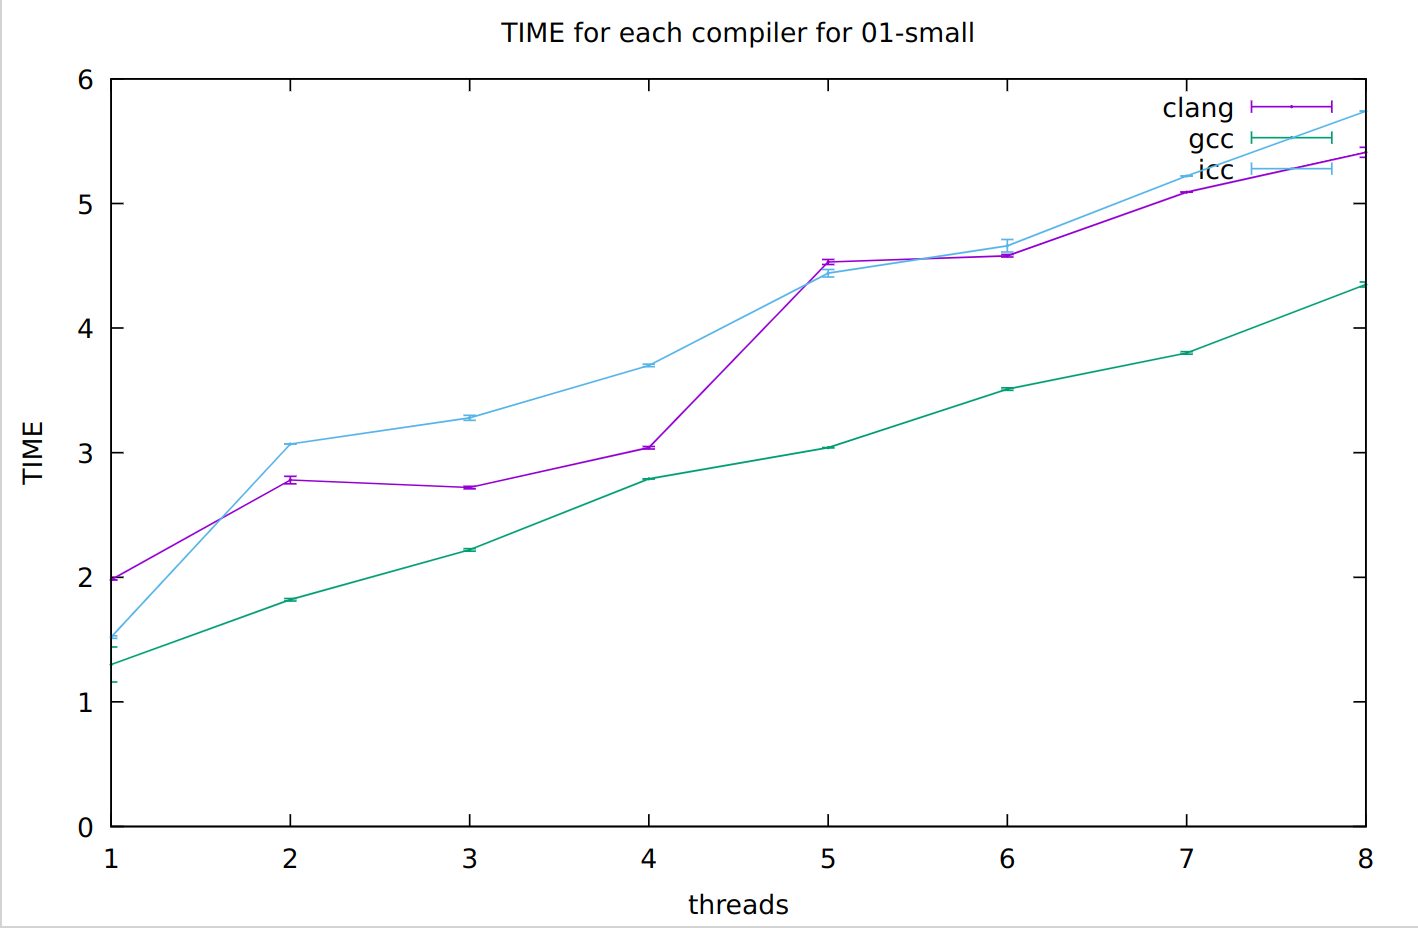
\includegraphics[width=\textwidth]{bucle3=01-small}
    \end{subfigure}
    \caption{\underline{Tamaño pequeño}: Tiempos de ejecución vs nº de hilos}
    \label{fig:bucle3=01-small}
\end{figure}

%%% TABLA DE TIEMPOS E IMÁGENES %%%
\begin{figure}[H]
    \centering
    \begin{subfigure}{0.4\textwidth}
        \begin{adjustbox}{width=\textwidth} 
        \begin{tabular}{|c|c|c|c|c|}
            \hline
            \rowcolor{azul} \multicolumn{2}{|c|}{}&\multicolumn{3}{c|}{\textbf{Compiler}} \\ \hline
            \rowcolor{azul} \multicolumn{2}{|c|}{}&\texttt{clang}&\texttt{gcc}&\texttt{icc}\\ \hline
            \rowcolor{azul} \textbf{Testing size} & \textbf{Threads}&\multicolumn{3}{c|}{\textbf{Average time (s)}} \\ \hline
            \multirow{8}{2.5cm}{\textbf{02-medium}} & 1 & \(5.29\pm{0.01}\) & \(2.05\pm{0.06}\) & \(3.87\pm{0.04}\) \\ \cline{2-5}
            & 2 & \(6.35\pm{0.02}\) & \(3.59\pm{0.03}\) & \(6.36\pm{0.05}\) \\ \cline{2-5}
            & 3 & \(5.78\pm{0.00}\) & \(4.24\pm{0.02}\) & \(6.71\pm{0.03}\) \\ \cline{2-5}
            & 4 & \(6.21\pm{0.01}\) & \(5.30\pm{0.02}\) & \(7.54\pm{0.04}\) \\ \cline{2-5}
            & 5 & \(8.94\pm{0.05}\) & \(6.17\pm{0.00}\) & \(9.16\pm{0.02}\) \\ \cline{2-5}
            & 6 & \(9.56\pm{0.19}\) & \(6.69\pm{0.01}\) & \(9.43\pm{0.04}\) \\ \cline{2-5}
            & 7 & \(10.31\pm{0.06}\) & \(7.64\pm{0.00}\) & \(10.33\pm{0.00}\) \\ \cline{2-5}
            & 8 & \(11.27\pm{0.00}\) & \(8.66\pm{0.03}\) & \(11.21\pm{0.02}\) \\ \hline
        \end{tabular}
        \end{adjustbox}
    \end{subfigure}
    \hfill
    \begin{subfigure}{0.5\textwidth}
        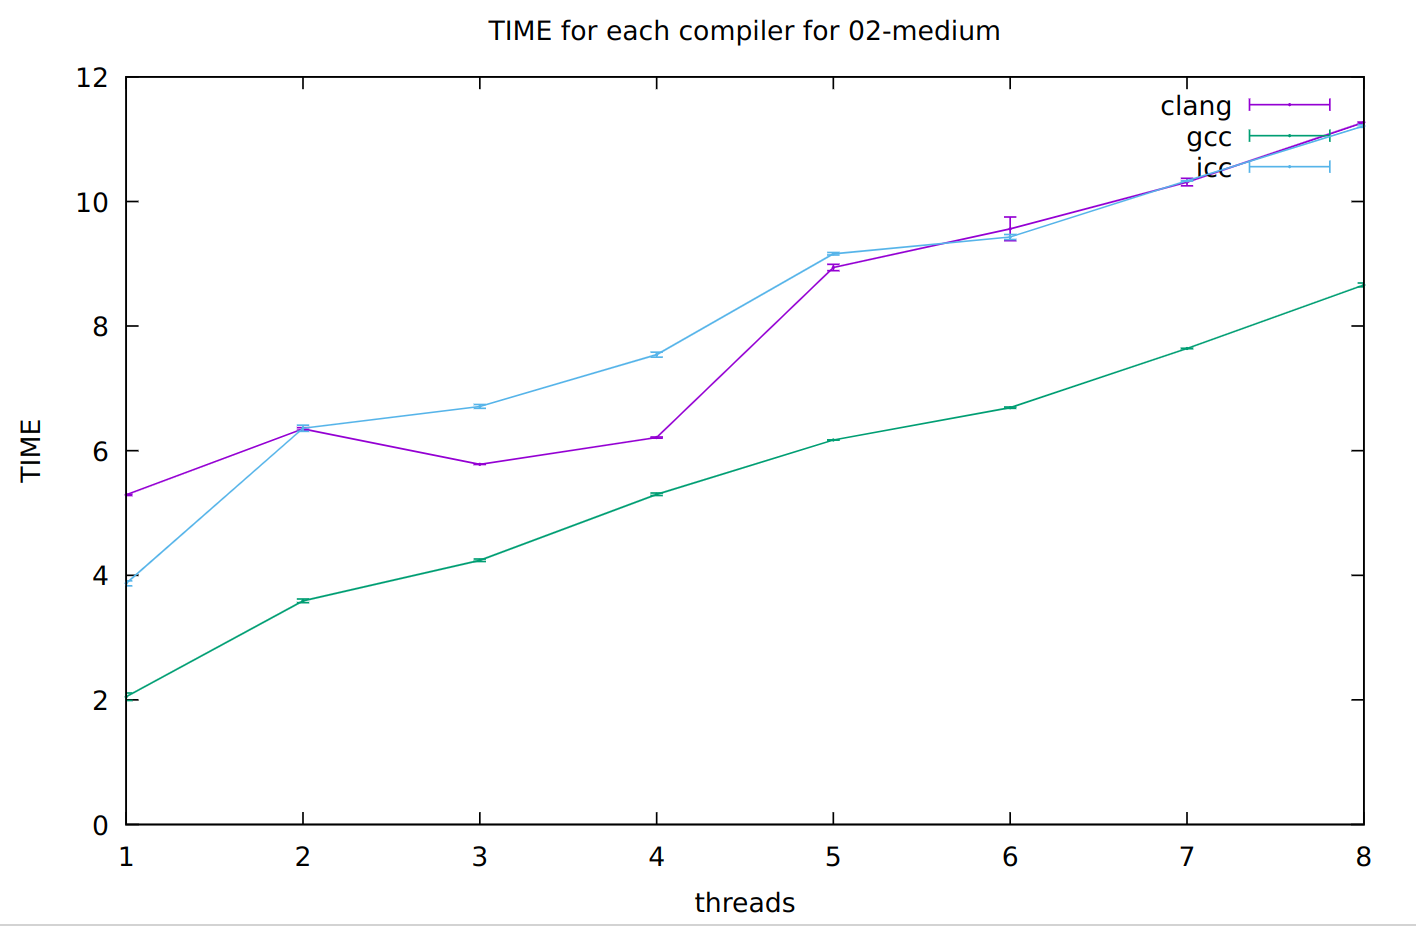
\includegraphics[width=\textwidth]{bucle3=02-medium}
    \end{subfigure}
    \caption{\underline{Tamaño mediano}: Tiempos de ejecución vs nº de hilos}
    \label{bucle3=02-medium}
\end{figure}

%%% TABLA DE TIEMPOS E IMÁGENES %%%
\begin{figure}[H]
    \centering
    \begin{subfigure}{0.4\textwidth}
        \begin{adjustbox}{width=\textwidth} 
        \begin{tabular}{|c|c|c|c|c|}
            \hline
            \rowcolor{azul} \multicolumn{2}{|c|}{}&\multicolumn{3}{c|}{\textbf{Compiler}} \\ \hline
            \rowcolor{azul} \multicolumn{2}{|c|}{}&\texttt{clang}&\texttt{gcc}&\texttt{icc}\\ \hline
            \rowcolor{azul} \textbf{Testing size} & \textbf{Threads}&\multicolumn{3}{c|}{\textbf{Average time (s)}} \\ \hline
            \multirow{8}{1cm}{\textbf{03-large}} & 1 & \(8.62\pm{0.04}\) & \(3.03\pm{0.11}\) & \(6.27\pm{0.16}\) \\ \cline{2-5}
            & 2 & \(8.98\pm{0.06}\) & \(3.03\pm{0.09}\) & \(8.94\pm{0.08}\) \\ \cline{2-5}
            & 3 & \(8.15\pm{0.07}\) & \(4.77\pm{0.05}\) & \(9.04\pm{0.11}\) \\ \cline{2-5}
            & 4 & \(8.25\pm{0.03}\) & \(6.09\pm{0.04}\) & \(9.92\pm{0.00}\) \\ \cline{2-5}
            & 5 & \(11.96\pm{0.09}\) & \(7.25\pm{0.02}\) & \(12.09\pm{0.08}\) \\ \cline{2-5}
            & 6 & \(12.23\pm{0.09}\) & \(8.06\pm{0.02}\) & \(12.84\pm{0.04}\) \\ \cline{2-5}
            & 7 & \(13.77\pm{0.04}\) & \(9.78\pm{0.03}\) & \(13.59\pm{0.05}\) \\ \cline{2-5}
            & 8 & \(14.93\pm{0.04}\) & \(10.70\pm{0.03}\) & \(14.98\pm{0.08}\) \\ \hline
        \end{tabular}
        \end{adjustbox}
    \end{subfigure}
    \hfill
    \begin{subfigure}{0.5\textwidth}
        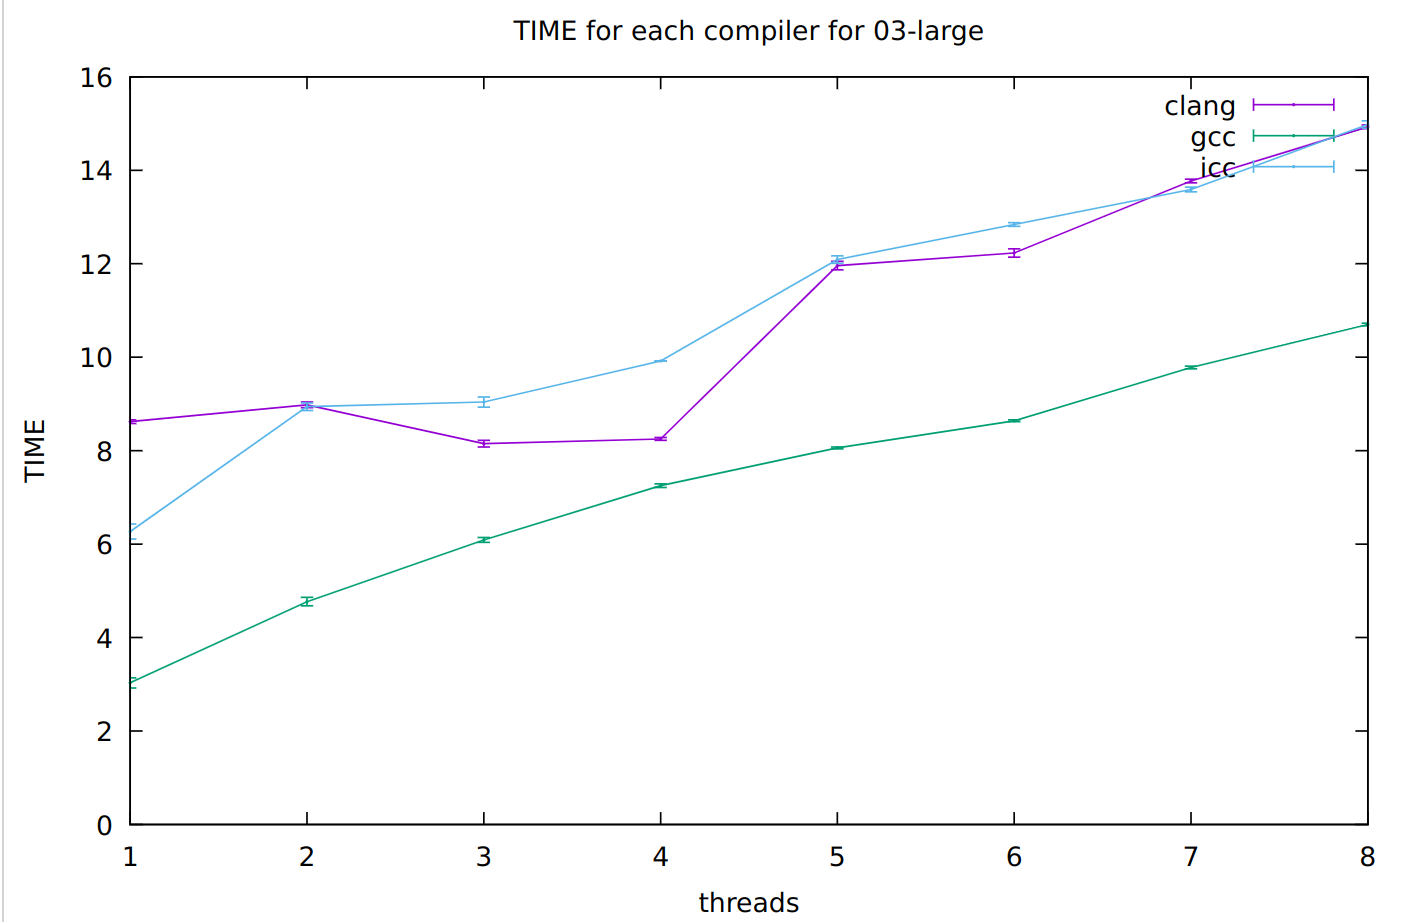
\includegraphics[width=\textwidth]{bucle3=03-large}
    \end{subfigure}
    \caption{\underline{Tamaño largo}: Tiempos de ejecución vs nº de hilos}
    \label{bucle3=03-large}
\end{figure}

\par Estos dos bucles anidados también podría ponerse el pragma \texttt{\#pragma omp parallel for collapse(2) reduction (max:difference)}
pero comprobando los tiempos se puede ver que empeora el tiempo de ejecución.
